\chapter{Related Work} 
\label{ch:relatedwork}

% This chapter should include a broad and detailed review of relevant existing
% work. The literature review
% should provide background and context for the thesis work. The subsections may be organized in whatever
% manner seems best suited to the material---chronological, or by topic, or
% according to some other criteria (e.g., primary versus secondary resources).

Automated fault localization in general and more specifically spectrum based
fault localization have extensive literature exploring the different approaches
to facilitate debugging and increase developer efficiency. Considering that
AFLuent relies on many concepts developed by this literature, this section will
explore and discuss how past work shapes AFLuent. Several sections are created
to for specific area of literature.

\section{Automated Fault Localization}
\label{sec:AFLlit}

Survey papers are one of the many ways that assist in better
understanding and having a wide collection of the existing
literature surrounding automated fault localization (AFL).
Wong et al. \cite{wong2016survey} explores the variety of AFL approaches and
surveys research completed in that area between 1977 and 2014. The survey paper finds and
discusses more than 334 different papers in many approaches in AFL.
\begin{figure}[!htb]
	\begin{center}
		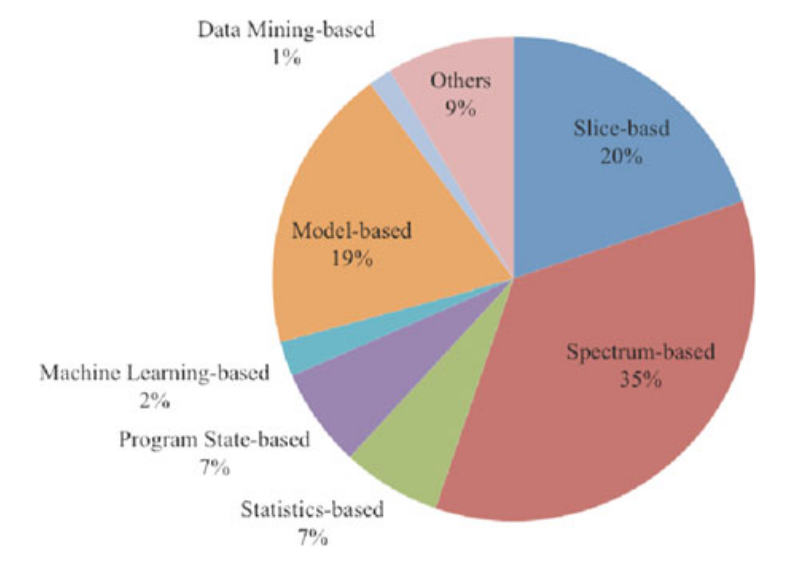
\includegraphics[width=10cm]{wong_pie_chart.png}
		\caption{\label{fig:wong_breakdown} AFL papers found by Wong et al. \cite{wong2016survey}}
	\end{center}
\end{figure}

A breakdown of the found research is shown in Fig. \ref{fig:wong_breakdown}, where the
majority of found papers are focused on Spectrum-Based Fault Localization (SFL).
Overall this research provides a great
starting point to find and compare the different types and approaches of AFL.
Another benefit of this resources is that
Wong et al. \cite{wong2016survey} expands on the types of SFL
and reviews key literature that contributes show the benefits and drawbacks of
each approach.

\subsection{SFL Approaches}
\label{subsec:sfl}

\subsubsection{Coefficient Based Technique}
\label{subsubsec:coefficient_based}
% TODO: add coefficient based table here

\subsubsection{Tarantula}
\label{subsubsec:tarantula_lit}

\subsubsection{Ochiai}
\label{subsubsec:ochiai_lit}

\subsubsection{DStar}
\label{subsubsec:dstar_lit}

\subsubsection{O and \textbf{$O^p$}}
\label{subsubsec:o_lit}

\subsection{Combining Approaches}
\label{subsec:combining_approaches}

While AFLuent does not rely on non-SFL approaches in its implementations, it's
useful to explore other methodologies that could assist in the debugging
process. This creates a guide for potential extendibility of AFLuent and
provides a way to fill in the shortcomings of AFLuent.
% TODO: develop more using "Search-based fault localization" and "Learning to Combine Multiple Ranking Metrics
% for Fault Localization"

\section{Existing Tools}
\label{sec:existing_tools}

\section{Usability and Accessibility}
\label{sec:usability_accessibility}

